\documentclass{report}

\usepackage{textcomp}
\usepackage{graphicx}
\usepackage{fancyhdr}
\usepackage{subcaption}
\usepackage{multicol}
\usepackage{outlines}
%===================================
\newcommand{\classinfo}{{\bf RHEL 134 \\ Week 03 Labs}\\{\it CIT 218}\\{Chaz Davis}}
\newcommand{\semester}{BCTC \\ Spring 2020}
%===================================
\newcommand{\mysection}[1]{\section*{#1}}
\newcommand{\mysubsection}[2]{\textbf{\romannumeral #1) #2}}
%===================================
\setlength{\headheight}{15.2pt}
\pagestyle{fancy}
\fancyhf{}
\lhead{ \fancyplain{}{Chaz Davis} }
\rhead{ \fancyplain{}{\today} }
\cfoot{ \fancyplain{}{\thepage} }
\renewcommand{\headrulewidth}{0.5pt}
\renewcommand{\footrulewidth}{0pt}

%===================================
\title{\classinfo}
\author{\semester}
\date{\today}

%===================================

\begin{document}

\maketitle

%===================================
\mysection{\textbf{Part 1: Questions}}


\mysubsection{1}{Create a file named “firstname\_lastname”. Set an ACL for your current user to have read-only access to the file. Provide the ACL details of the file.}\\
I created a directory named chaz with the command 
{\scriptsize{\verb$mkdir chaz$}\normalsize} and then cd'd into the directory. 
I then created a file names Chaz\_Davis.txt with the command
{\scriptsize{\verb$touch Chaz_Davis.txt$}\normalsize} then set the acl for the
user using the comnmand
{\scriptsize{\verb$setfacl -m u::rX Chaz_Davis.txt$}\normalsize}, where the
{\scriptsize{\verb$-m$}\normalsize} means to modify and the
{\scriptsize{\verb$u::rX$}\normalsize} means that for the default user let this
file be read-only and remove execution permissions unless explicitly stated,
for this file and recursively through directories. this isn't a necessary step,
but is considered best practice. I then viewed the output of the act by running
the command {\scriptsize{\verb$getfacl Chaz_Davis.txt$}\normalsize}. You can
see the Screenshot in Fig.~\ref{Wk02}\subref{Wk02Q01} on Pg.~\pageref{Wk02}.


\noindent\mysubsection{2}{Create a directory named “CIT218” in your home directory. Set an ACL to allow recursive read/write access on the directory for the “student” group. Provide the ACL details of the directory.}\\
From my jome directory I created a directory named "CIT218" by running the
command {\scriptsize{\verb$mkdir CIT218$}\normalsize}, and then I set an ACL
for that directory by running 
{\scriptsize{\verb$setfacl -R -m g:student:rw CIT218$}\normalsize}, where
{\scriptsize{\verb$-R -m$}\normalsize} means modify the acl Recursively, and
then {\scriptsize{\verb$g:student:rw$}\normalsize} means for group student,
restrict access to read and write only. I then checked the acl config by
running {\scriptsize{\verb$getfacl CIT218$}\normalsize}. See the Screenshot in
Fig.~\ref{Wk02}\subref{Wk02Q02} on Pg.~\pageref{Wk02}.


\noindent\mysubsection{3}{Change the mode of SELinux to disabled. Provide the output.}\\
I logged in as root and typed 
{\scriptsize{\verb$vi /etc/selinux/config$}\normalsize}, once in vi i went to
the line with {\scriptsize{\verb$SELINUX=enforcing$}\normalsize} and changed it
to {\scriptsize{\verb$SELINUX=disabled$}\normalsize}, I then saved my work with
{\scriptsize{\verb$:wq$}\normalsize}. Once back in the terminal i checked the
output by typing {\scriptsize{\verb$cat /etc/selinux/config$}\normalsize}. You
can see the ouput in Fig.~\ref{Wk02}\subref{Wk02Q03} on Pg.~\pageref{Wk02}.



\noindent\mysubsection{4}{Create a file named “firstname\_lastname”. Change the
file context to httpd\_sys\_content\_t.  Provide the SELinux details of the file.}\\
I logged into the terminal as root and installed the apache server by running
{\scriptsize{\verb$yum -y install httpd$}\normalsize}. Next, I created the file
Chaz\_Davis by running {\scriptsize{\verb$touch Chaz\_Davis$}\normalsize}. I
then changed the selinux context for the file by using
{\scriptsize{\verb$chcon -t httpd_sys_content_t Chaz_Davis$}\normalsize}, i
could have also done this with 
{\scriptsize{\verb$semange fcontext -t httpd_sys_content_t Chaz_Davis$}\normalsize},
which I believe is technically the preferred method fo management fo the
context of a file. I then got the configuration of the file output in the
terminal by running
{\scriptsize{\verb$ls -Z Chaz_Davis$}\normalsize}. You can see in
Fig.~\ref{Wk02}~\subref{Wk02Q04} 
on Pg.~\pageref{Wk02}.



\noindent\mysubsection{5}{Allow the HTTPS service through the firewall. Make it permanent and reload the firewall. }\\
I started off by logging into the terminal as root, I then ran the comnmand
{\scriptsize{\verb$firewall-cmd --permanent --zone=public --add-service=https$}\normalsize} 
, I then ran {\scriptsize{\verb$firewall-cmd --reload$}\normalsize}, and
finally to check that it stuck I ran {\scriptsize{\verb$firewall-cmd --list-all$}\normalsize} 
You can see in Fig.~\ref{Wk02}~\subref{Wk02Q05} 
on Pg.~\pageref{Wk02}.


\begin{figure}[!hbt]\centering
\subfloat[Setting ACL for File]{\label{Wk02Q01}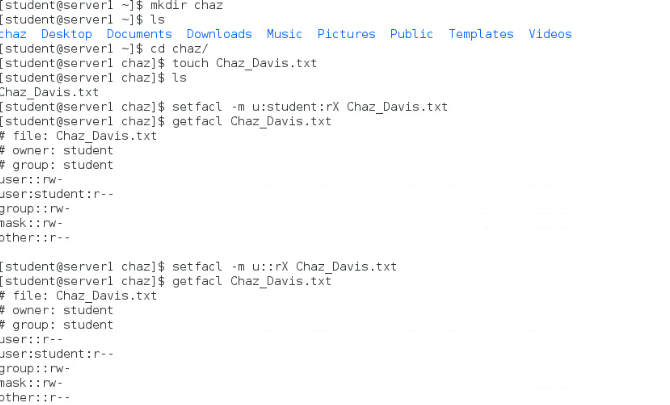
\includegraphics[width=.65\linewidth]{Figures/Q01.png}}\par
\subfloat[Setting ACL for Directory]{\label{Wk02Q02}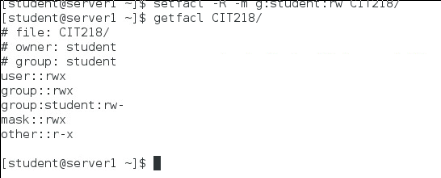
\includegraphics[width=.49\linewidth]{Figures/Q02.png}}\hfill
\subfloat[Disabling Selinux]{\label{Wk02Q03}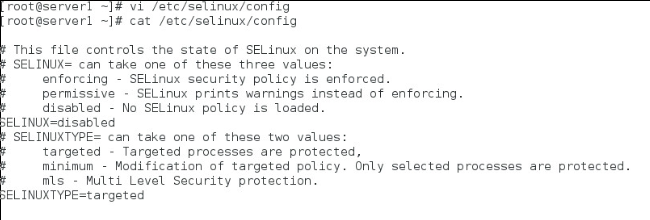
\includegraphics[width=.49\linewidth]{Figures/Q03.png}}\par
\subfloat[Changing Selinux context of a file]{\label{Wk02Q04}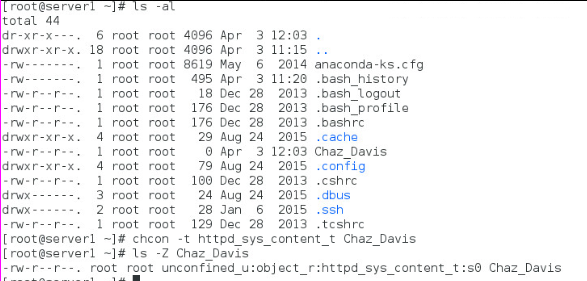
\includegraphics[width=.49\linewidth]{Figures/Q04.png}}\hfill
\subfloat[Allowing HTTPS through the firewall]{\label{Wk02Q05}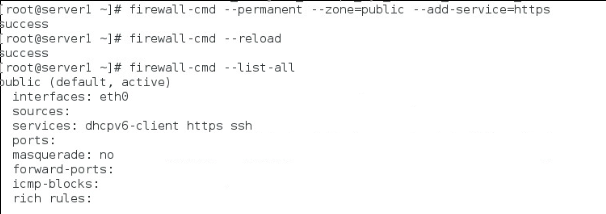
\includegraphics[width=.49\linewidth]{Figures/Q05.png}}\par
\caption{Screenshots for Week 3 Labs}\label{Wk02}
\end{figure}



%===================================

\end{document}
